\section{Демодулятор}
Задача демодулятора восстановить информационный (модулирующий) сигнал из принятого искаженного. Вследствие неидеальности канала, оборудования у нас возникают искажения различных типов - аддитивный гауссовый шум, частотная рассинхронизация, межсимвольная интерференция, многолучевое распространение.
На рис.23 приведена структурная схема идеального демодулятора, содержащего квадратурный демодулятор и ряд преобразователей, формирующих передаваемую цифровую информацию.
В квадратурном демодуляторе входной сигнал можно представить в таком виде, где I(n)  и Q(n)  - синфазная и квадратурные составляющие,$f_u$ - частота несущей $$S(t)  = I(t)+ iQ(t) $$
 Он перемножается с двумя
сдвинутыми на $ \frac {\pi}{2}$ синусоидальными сигналами опорной частоты $f_s$ 
На АЦП поступают две составляющие сигнала, квадратурная (${U_q}$) и синфазная(${U_i}$): $$U_{i} = (I(t)(\cos{2 n \pi f_s t} - Q(t)(\sin{2 n \pi f_s t} ) )$$$$U_{q} =(I(t)(\sin{2\pi f_s t} + Q(t)(\cos{2 \pi f_s t} ) ), 
$$
Поданный на вход блока БПФ (быстрое преобразование Фурье) сигнал можно представить в таком виде:  $$U(t) = U_{bi}(t) + U_{bq}(t) = \sum_{n=1}^{2N+1}(I(n) + j Q(n))exp(j2\pi f_u t)$$, то после преобразования получим просто $S(n) = I(n) + j Q(n)$ , где $I(n)\ и\ Q(n)$ - те значения, которые подавались на модулятор.
\begin{figure}[h]
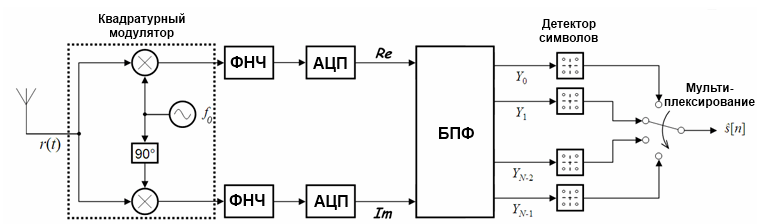
\includegraphics{demod}
\caption{схема идеального демодулятора}
\end{figure}


\subsection{Синхронизация}



\subsubsection{Временная}
Демодулятор начинает работу в произвольный момент времени, из -за чего сперва необходимо определить начало первого целого символа  OFDM, иначе декодировать данные не удастся.

\paragraph{Грубая}
Автокорреляционный метод анализа основан на совпадении структур сигнала, расположенные в защитном и активном интервалах передаваемого символа.

Для этой цели используется скользящее окно, состоящее из двух активных областей (стробов), разнесенных на длительность активного интервала. Длительность каждого строба (n отсчетов) скользящего окна выбирается меньше длительности защитного интервала (M отсчетов, M < n ).

Значения коэффициентов автокорреляционной функции будут наибольшими в случае
максимальной похожести сигналов $S_1(n)$ и $S_2(n)$, расположенных в активных областях  скользящего окна:
$$R = \sum_{i=1}^{n}S_1 S_2^* =
\begin{cases}
R_{max}, & \text{если $ S_1  = S_2 $;} \\
r R_{max},r < 1 & \text{если $ S_1 \neq S_2 $.}
\end{cases} $$
Таким образом, автокорреляционная функция будет иметь некоторое плато или пик в зависимости от длины защитного интервала, Для более точного вычисления можно использовать усреднение по нескольким символам OFDM. 
\begin{figure}[!h]
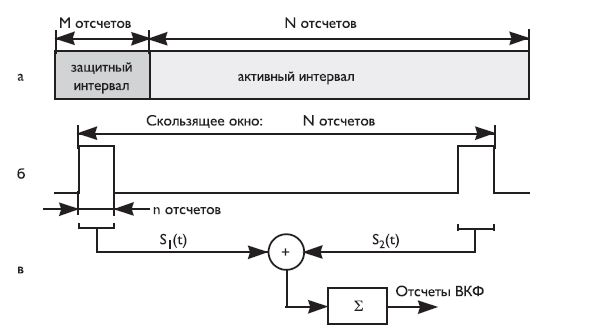
\includegraphics{correl}
\caption{применение автокорреляции}
\end{figure}

\paragraph {Тонкая}
В зависимости от того, в какое место защитного интервала мы встали, АЧХ нашего символа не будет изменяться, но на ФЧХ будет произведено действие, аналогичное  действию оператора сдвига.
\begin{figure}[!h]
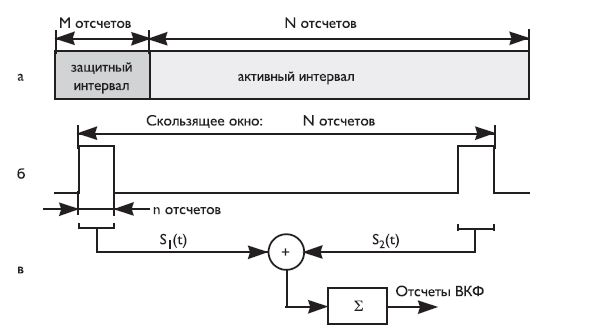
\includegraphics{correl}
\caption{вид закрученного созвездия}
\end{figure}
Если сейчас  взглянуть на созвездие (примерный вид на картинке), то можно увидеть, что оно закручивается (по или против часовой стрелки в зависимости от того, префиксный защитный интервал или постфиксный) - это есть набег фаз в результате действия оператора сдвига. Так как оператор сдвига линеен и известны фазы пилотов, мы можем аппроксимировать фазы информационных отсчетов между пилотами. 
Здесь существует одна тонкость: так как значения углов лежат в диапазоне $[0:2 \pi]$, то если набег фазы будет больше $2\pi$, то ФЧХ в этом месте будет совершать скачок: таким образом, мы должны следить за монотонностью интерполирующей прямой и при необходимости корректировать набег на $2\pi$. 
$\Delta \phi = \phi_k + 2\pi k - \phi_n-2\pi n = (\omega_k - \omega_n)\Delta t+ 2\pi (n-k)$

\subsection {Частотная}
Также одной из проблем реализации систем с использованием OFDM--модуляции является слежение за подстройкой частоты дискретизации сигналов при выполнении БПФ. В силу ряда причин (например,  приемник и передатчик могут быть не строго синхронизированы) номинальные частоты спектральных составляющих OFDM--сигнала могут не совпадать с соответствующими частотами гармоник БПФ, как показано на рис.25. Дискретизация принимаемого сигнала с частотой, отличающейся от номинальной величины, является причиной снижения точности восстановления модулированных символов, передаваемых на каждой поднесущей.

Оценка величины частотного смещения $\Delta f $ осуществляется с применением автокорреляционной функции с использованием заложенной в OFDM--сигнал избыточности в виде защитного интервала.

\begin{figure}[!h]
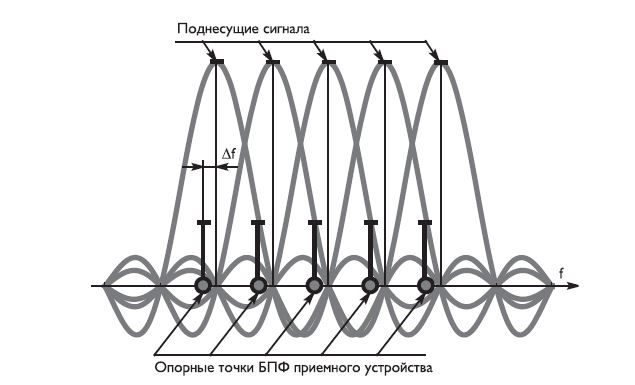
\includegraphics{freqDesync}
\caption{частотное смещение в принятом сигнала}
\end{figure}


$R = \sum_{i=1}^{n}S_1 S_2^* exp{(i(f_1 - f_2 + \Delta f )}$. Очевидно, что автокорреляционная функция будет "убивать" одинаковые частоты, попадающие в скользящее окно, оставляя $\Delta f $  --- величину частотной рассинхронизации.  


\subsubsection{Эквалайзинг}

\paragraph {Назначение}
Как уже говорилось раннее, многолучевое распространение присутствует в большинстве радиолиний. Явление многолучевого распространения может вызвать флуктуации амплитуды, фазы и угла прибытия, что приводит к эффекту замирания. Для борьбы с замираниями используется выравнивание - эквалайзинг. Картину сигнала после канала с замираниями можно посмотреть в соответствующей главе.
По сути, эквалайзер есть  восстановление импульсной характеристики канала и использование ее для компенсации искажений. Если канал является частотно-селективным, эквалайзер усиливает частотные компоненты с малыми амплитудами и ослабляет с большими. Целью комбинации канала и выравнивающего фильтра является получение ровной частотной характеристики и изменения фазы. 

\paragraph {Математика}

\begin{figure}[!h]
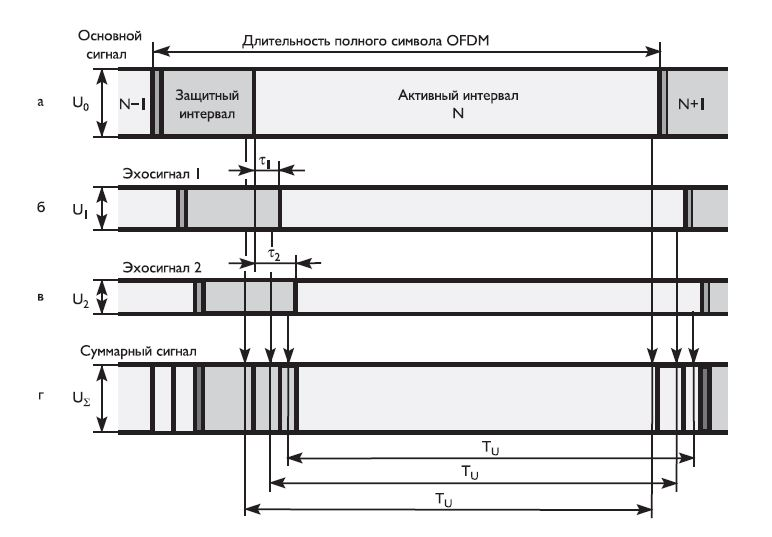
\includegraphics{manyRays}
\caption{сигнал в многолучевом сигнале}
\end{figure}

Прохождение сигнала по каналу можно описать как: $$r(t) = s(t)\circledast h(t)$$ где r(t) - выходной сигнал, s(t) - входной сигнал, h(t) - испульсная характеристика канала. Согласно теореме о свертке, свертка во временной области есть перемножение в частотной:  $$R(f) = S(f) H(f)$$ где H(f) - частотная характеристика канала, S(f) - спектр сигнала на входе. Здесь возможно воспользоваться знаниями об АЧХ пилотов и восстановить  с ее помощью АЧХ всего сигнала.
Необходимо добавить, что так как частотная характеристика канала может оказаться нелинейной,линейной аппроксимации будет недостаточно.

\subsubsection {реформирование созвездия} 
Реформирование созвездия и формирование битовой последовательности (демаппинг)  - процесс принятия решения, может быть либо {\bf жёстким}, либо {\bf мягким}. 
Чтобы лучше понять идею можно рассмотреть случай, когда двоичный сигнал передается за отрезок времени Т, причем двоичная единица представляется сигналом $s_1(t) $, а двоичный нуль — сигналом $s_2(t) $. 
Принятый сигнал имеет вид $r(t) = s(t)+n(t) $, где n(t) представляет собой вклад гауссового шума с нулевым средним. так как n(t) — это случайная переменная c нулевым средним, то и r(t) будет случайной гауссовой величиной со не нулевым средним. Затем принимается решение о том, какой сигнал был передан на основе сравнения r(T) с порогом $p(r|s_1)$. Условные вероятности , показанные на рисунке, обозначены как правдоподобие  $s_1(t) $ и$s_2(t) $ . Демодулятор преобразует упорядоченный по времени набор случайных переменных  в кодовую последовательность Z и подает ее на декодер. Выход демодулятора можно настроить по-разному. Можно реализовать его в виде {\bf жёсткой} схемы принятия решений --- в этом случае выход демодулятора квантуется на два уровня,0 и 1, и соединяется с декодером.
\begin{figure}[h]

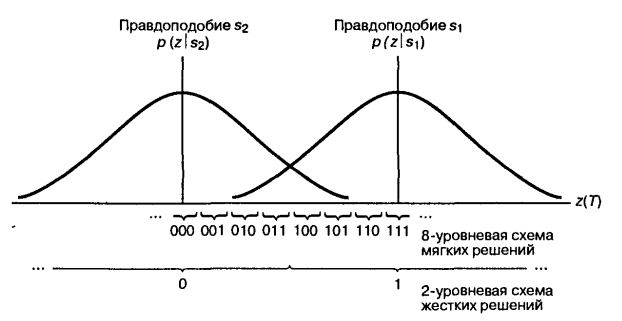
\includegraphics{decision}
\caption{жесткая и мягкая схемы декодирования}
\end{figure}
В другом случае демодулятор можно настроить так, чтобы он подавал на декодер значение r(T), квантованное более чем на два уровня. Такая, {\bf мягкая}, схема обеспечивает декодер большим количеством информации, чем жесткая схема решений. На рис. 7.8 на оси абсцисс изображено восемь (3-битовых) уровней квантования. Если в демодуляторе реализована жесткая схема принятия двоичных решений, он отправляет на декодер только один двоичный символ. Если в демодуляторе реализована мягкая двоичная схема принятия решений, квантованная на восемь уровней, он отправляет на декодер 3-битовое слово, описывающее интервал, соответствующий r(t). По сути, поступление такого 3-битового слова, вместо одного двоичного символа эквивалентно передаче декодеру меры достоверности вместе с решением относительно кодового символа.

Согласно рисунку последовательность 111 равносильна тому, что с очень высокой степенью достоверности кодовым символом была 1, когда последовательность 100 означает, что  1 была с очень низкой степенью достоверности. Разумеется, в конечном счете каждое решение, принятое декодером, должно быть жестким в силу устройства компьютера. То, что после демодулятора не принимается жесткое решение и на декодер поступает больше данных (мягкое принятие решений), можно понимать как промежуточный этап, необходимый для того, чтобы на декодер поступило больше информации, с помощью которой он затем сможет восстановить последовательность сообщения (с более высокой достоверностью передачи сообщения по сравнению с декодированием в рамках жесткой схемы принятия решений). Показанная на рис. , 8-уровневая метрика мягкой схемы принятия решений часто обозначается как -7, -5, -3, -1, 1, 3, 5, 7. Такие обозначения вводятся для простоты интерпретации мягкой схемы принятия решения. Знак метрики характеризует решение (например, выбирается  $s_1(t) $ , если величина положительна, и  $s_2(t) $, если отрицательна), а величина метрики описывает степень достоверности этого решения.


